\documentclass[12pt]{article}
%\documentclass[8pt,twocolumn]{article}

\usepackage[letterpaper, margin=0.75in]{geometry}
\usepackage{graphicx}
\usepackage{comment}
\usepackage{float}
\usepackage{hyperref}
\usepackage[authoryear]{natbib}
\usepackage{setspace}
\usepackage{mathtools}
\usepackage{subcaption}
%\usepackage{aas_macros}
\usepackage{amssymb}
\usepackage{textcomp}
\usepackage{siunitx}

%\onehalfspacing
\doublespacing

\title{The Aerosol Limb Imager: Acousto-Optic Measurements of Limb Scattered Sunlight for 2D Stratospheric Aerosol Profiles}

\author{Brenden J Elash, Adam E Bourassa, Paul R P Loewen, Douglas A Degenstein}

\begin{document}
\renewcommand\bibname{BiBTex.bib}

\maketitle

\abstract{The Aerosol Limb Imager (ALI) is a remote sensing instrument developed at the University of Saskatchewan, Canada, for measurement of scattered sunlight from the atmospheric limb to retrieve spatially resolved information of the stratospheric aerosol distribution, including extinction coefficient and particle size. The long term goal of this work is the eventual realization of ALI on a satellite platform in low earth orbit. Here we present the development of an ALI prototype and the results from a test flight on a stratospheric balloon. The ALI instrument concept uses a large aperture Acousto-Optical Tunable Filter (AOTF) to successively image the stratospheric limb in a selectable narrow wavelength band from the visible to the near infrared. The afocal optical system design uses telescopic front end optics to pass collimated light through the AOTF for each line-of-sight, which provides robust imaging that is relatively insensitive to impurities in the AOTF, at the cost of a small spectral gradient in the measured image that is negligible for the broad band aerosol spectral scattering characteristic. The ALI prototype was tested on a stratospheric balloon flight from the Canadian Space Agency (CSA) launch facility in Timmins, Canada, in September, 2014. Preliminary analysis of hyperspectral images indicate that the radiance measurements are high quality and can be used to retrieve vertical profiles of stratospheric aerosol extinction coefficient and one moment of the particle size distribution.}

\section{Introduction}
\label{sec:introduction}

Sulfuric aerosol is a fundamental portion of the global climate balance. Aerosol is a spherical particle consisting of hydrated droplets of sulfuric acid that scatters incoming radiance away from the surface of the planet causing an overall cooling effect which is dependant on extinction and particle size distribution \citep{Kiehl1993}. This effect is fully defined by aerosol microphysics requiring accurate knowledge of concentration and particle size distributions. Stratospheric aerosol loading has been increasing at a rate of 4-7\% per year from 2002 to 2009 due to moderate volcanic eruptions \citep{Vernier2011} which have lead to a negative radiative effect that has potentially partially offset the radiative forcing from CO$_{2}$ \citep{Solomon2011}.  The method of aerosol transportation across the tropopause are not completely understood. Recently, the 2011 eruption of Nabro ejected  SO$_{2}$ into the troposphere which was transported into the anticyclone of the asian monsoon. The monsoon vertically transported the aerosol across the tropopause into the stratosphere \citep{Bourassa2012c}. The Asian summer monsoon performs this transportation through its large scale anticyclone circulation that propels atmospheric constituents upwards and isolates it from the external environment. Also anthropogenic sources of SO$_{2}$ can enter the stratosphere through the Asian tropopause aerosol layer that forms during the Asian monsoon \citep{Vernier2011, Neely2014}.

Aerosol in the stratosphere has been monitored via remote sensing applications throughout the last few decades. Solar occultation has been the method used the longest to monitor aerosol in the stratosphere and has built up a reliable, accuracy and long term database of background and volcanic aerosol extinctions. Notable occultation instruments include SAM II \citep{McCormick1979}, SAGE II \citep{McCormick1987}, and SAGE III \citep{Thomason2003} with combined life cycles gathered measurements from 1978 to 2005. The occultation method has the ability to self-calibrate each measurement by directly viewing the sun outside of the atmospheric giving stable profiles. The method also directly measures the optical depth allowing for simple conversion to extinction without the the need for particle size knowledge.

More recently the limb scatter geometry, which measures scattered radiance from the sunlit atmosphere, has been used to determined aerosol extinction. Although this geometry has the advantage of being able to measure the atmosphere in any sunlit conditions, unlike occultation which can only gather measurements during sunrise or sunset events. The scattering process requires the use of a forward model to determine atmospheric parameters, making determining atmospheric species from limb geometry computationally heavy and time intensive. Limb scatter was first preformed on the Solar Mesosphere Explorer (SME) \citep{Barth1983} to measure ozone profiles in 1981 and was followed by instruments with the ability to measure aerosol. The Optical Spectrograph and InfraRed Imaging System (OSIRIS) a Canadian instrument onboard the Odin satellite \citep{Llewellyn2004} and SCanning Imaging Absorption spectroMeter for Atmospheric CHartographY (SCIAMACHY) onboard the ENVISAT \citep{Bovensmann1999} are two limb scatter instruments have successfully determined aerosol atmospheric parameters. These instruments grating spectrometers that acquire data at a single tangent altitude at a time so a series of exposures is required to create a vertical profile with approximately a 1.5~km and 3~km vertical resolution for OSIRIS and SCIAMACHY respectively. The Ozone Mapping Profiler Suite - Limb Profiler (OMPS-LP) \citep{Rault2013} uses a prism to disperse the light and images the atmosphere through three verticals slits. Each slit images 100~km vertically with a 1.5~km resolution and the center slit look backward along the satellite track and the other two slits are offset by 4.25\si{\degree} horizontally which increases the amount of data that can acquire in a single orbit.

A future generation limb instrument would also require higher vertical and resolution than current limb instruments. A lidar instrument, CALIPSO, is able to achieve aerosol profiles of 333~m horizontal resolution and 60~m, 180~m, and 300~m vertical resolution for the altitude ranges of 8.2-20.2~km, 20.2-30.1~km, and 30.1-40.0~km respectively \citep{Winker2003}. The aerosol product is a 16 day average 3-D grid with a resolution of 1\si{\degree} latitude by 2\si{\degree} longitude by 200~m vertically. Each aerosol data grid is the average of 300 to 600 profiles \citep{Vernier2009}. Additional instrumentation with high resolutions on the order of 200~m vertically will satisfy the needs for current scientific investigation and will allow the determination of aerosol loading.

ALI, a prototype for a next generation of instruments will address the much needed horizontal and vertical resolution. ALI will used the limb scatter geometry to gather 2-D spacial images of the atmosphere and uses an Acousto-Optic Tunable Filter (AOTF) which is a device that allows the change of a filtering wavelength without any moving parts and low power consumption. AOTFs have good operation characteristics in the Near InfraRed (NIR) which allows for good device to measure aerosol signal. Inherently, AOTFs can only filter linearity polarized signal making ALI a polarized instrument. Further the bandpass of the AOTF, approximately 2~nm at 600~nm and 7~nm at 1100~nm, align well with the broadband scattering characteristic of the aerosol signal. ALI will measure scattered sunlight form 650-950~nm with a stratospheric balloon flight from Timmins Ontario in the fall of 2014.

A similar instrument, the Atmospheric Limb Tracker for the Investigation of the Upcoming Stratosphere (ALTIUS) is designed by Belgium and its goal is to measure trace gas concentrations from measuring light in the limb scatter geometry as well as solar stellar, and planetary occultation \citep{Dekemper2012}. ALTIUS images the atmosphere with 2 spacial directions like ALI and also used AOTFs has the filtering device. ALTIUS is a multichannel instrument using three AOTFs with different wavelength bands. The three channels for ALTIUS are an ultraviolet, viable, and NIR with wavelength ranges of 250-450~nm, 450-900~nm, and 900-1800~nm respectively.

In this paper, the first section will outline the technology behind the AOTF used within the ALI system. Following is a description of the optical design behind ALI including an ulterior optical presentation comparing the benefits and drawbacks between two optical layouts. An overview of ALI's maiden flight, including the conditions and trajectory of the flight, onboard the CNES CARMEN-2 gondola from the CSA balloon launch facility in Timmins, Ontario will be presented. Post flight analysis of the data is presented including the measurements taken during the campaign, the conversion from raw measurements into calibrated data, and an retrieval algorithm for aerosol extinction and particle size parameters will be outlined and then preformed on the data from the campaign.

\section{Instrument Design}

\subsection{Acouto-Optical Tunable Filter}

The primary filtering device behind ALI and the technology that allows two dimensional spacial imaging is the AOTF. It uses an acoustic wave, which frequency is determined by a Radio Frequency (RF), that is propagated through the crystal and forms a standing wave to allow an effect similar to diffraction of a specific wavelength causing a filtering effect. The use of an AOTF for an imaging system has several distinct advantages due to its low mass, fast stabilization times of a few microseconds, no moving parts. Non-collinear acousto devices with the use of birefringent materials with large apertures are used in imaging systems \citep{Chang1974}. Thanks to recent advancements of non-collinear AOTF technology these devices can be used in imaging systems \citep{Georgiev2002, Voloshinov2007}. In order for the AOTF to allow the diffraction of a specific wavelength a momentum matching criteria must be held where the wave vectors of the acoustic wave match the difference of the incoming and diffracted light wave vectors as seen in \autoref{fig:3.1:ATOFWavevectors}. This condition is known as the Bragg matching criteria and is given by
\begin{equation}
    \ \mathbf{k}_{i} = \boldsymbol\kappa + \mathbf{k}_{d}
    \label{eqn:3.1:phaseMatching}
\end{equation}
where $\left|\mathbf{k}_{i}\right| = \frac{2\pi n_{i}}{\lambda}$ is the wave vector of the incoming light, $\left|\mathbf{k}_{d}\right| = \frac{2\pi n_{d}}{\lambda}$ is the momentum of the diffracted light, and $\left|\boldsymbol\kappa\right| = \frac{2\pi F}{\nu}$ is the momentum of the acousto wave. The parameters $\lambda$, $F$, and $\nu$ are the wavelength in vacuum, the frequency of the RF wave, and the phase velocity in the crystal respectively. Using the condition given in \autoref{eqn:3.1:phaseMatching} and the wave vector diagram gives the following relation for a birefringent material undergoing Bragg diffraction
\begin{equation}
    \lambda  = \frac{\Delta n\nu}{F}\frac{\sin^{2}(\theta_{i}+\alpha)}{\sin\theta_{i}}
    \label{eqn:3.1:AOTFWavelengthDependance}
\end{equation}
where $\Delta n$ is the absolute difference between the ordinary and extraordinary indices of refraction, $\theta_{i}$ is the angle of incidence of the incoming light, and $\alpha$ is the angle the acoustic wave propagates though the device. This equation has several implications to the operation of the device, first the wavelength diffracted by the AOTF is inversely related to frequency of the RF wave. Second the wavelength of outgoing signal is dependant the angle of incidence of the incoming wave therefore passing a signal though the AOTF at different incident angles will result in a different outgoing wavelength which will cause a consideration for any optical design. Also, through the described interaction the diffracted light goes though a 90\si{\degree} rotation in polarization \citep{Voloshinov1996}.

A 10x10~mm aperture imaging quality ATOF was acquired from Brimrose of America. It is optically tuned, meaning designed for a specific wavelength octave, for a range of 600 to 1200~ nm corresponding to a RF range of 156 to 70~MHz and made from Tellurium Dioxide (TeO$_{2}$), a birefringent crystal with indices of refraction at 800~nm of 2.226 and 2.373 for the ordinary and extraordinary modes respectively \citep{Uchida1971}. The extraordinary light is diffracted at 2.7 degrees off of the optical axis of the device. In order to achieve a constant diffraction angle of the first order beam a wedge is attached to the exit aperture of the AOTF to compensate for the angular change that occurs from altering the wavelength. The ordinary light undergoes diffraction but at a nonconstant angle off of the optical axis with respect to wavelength due to the ordinary polarization being uncompensated. It is important to note that it is currently not possible to have both polarizations compensated and as such only the extraordinary polarization is captured by ALI.

\subsection{AOTF Characterization}

Characterization of the AOTF is required for calibrated use in an instrument. For characterization, the AOTF used in an optical system that allows the best determination of the central wavelength of the device. In this system linear polarizers were inserted before and after the AOTF to remove undesired signals. A 100~mm plano-convex lenses were chosen for the front and back end lenses to best fill the AOTF aperture. The light source is a 100~W quartz-tungsten halogen bulb that is collimated and passed into the first lens. The light passes though the AOTF focused then is re-collimated through the second lens. The signal enters a HORIBA iHR320 spectrometer with a minimum spectral resolution of 1.175~nm. The spectral results were imaged on a Synapse 354308 front-illuminated CCD detector with 1024x256 pixels. Images were taken at a set of RFs spaced every 150~kHz from 75~MHz to 160~MHz. For each image the results are spectrally averaged across the rows and a typical spectral measurement result can be seen in \autoref{fig:3.1:AOTFCharaterization:a}. The maximum value of each image is taken to be the central wavelength through the AOTF at each respective RF.

The maximum values from each of the images were determined as well as the corresponding wavelengths for these values. It was noted that the curve appears to follow a power function of the form
\begin{equation}
    \ F = a\lambda^{b}.
    \label{eqn:3.1:powerFunction}
\end{equation}
A linear least squares fit was preformed in log space finding the coefficients $a$ and $b$. The fit provided an agreement better than 0.6\% within the testing range. A better fit was found in the form of
 \begin{equation}
    \ F = a\lambda^{b+c\log\lambda}.
    \label{eqn:3.1:modifiedPowerFunction}
\end{equation}
These results can be seen in \autoref{fig:3.1:AOTFCharaterization:c} and \autoref{fig:3.1:AOTFCharaterization:d}. The agreement of this form is less than 0.1\% throughout the whole wavelength range and the determined RF and wavelength relation can be seen in
\begin{equation}
    \ F = \exp{(19.793)}\lambda^{-3.381+0.168\log\lambda}
    \label{eqn:3.1:modifiedPowerFunctionCoeffiecicents}
\end{equation}
where $\lambda$ is in nanometers and $F$ is in MHz. It should be noted that even though the AOTF optical range is 600~nm to 1200~nm this analysis only measures wavelengths from 600~nm to 1080~nm. The low quantum efficiency of the CCD and the low near IR emitted from the light source causes this form to be limited to wavelengths less than 1000~nm.

The same set of data was used to determine the Full Width Half Max (FWHM) for each of the above determined wavelengths. The results of this study are shown in \autoref{fig:3.1:AOTFCharaterization:b}. However, the AOTF spectral resolution is well within the limits that are required in order to determine aerosol extinction in the upper troposphere and lower stratosphere which is discussed under the \autoref{sec:introduction}.

The diffraction efficiently was determined using two sets of data; the first set is the data used to characterize the wavelength-RF dependance of the AOTF, the second set is a measurement of the light that was incident to the AOTF in the previous experiment. To acquired the incident data the AOTF and linear polarizer on the back end of the optical chain was removed. The light source is measured again with the spectrometer without the diffraction of the AOTF. By taking the ratio of the diffracted wavelength over the incident radiance the diffraction efficacy was determined. The determined diffraction efficiency is between 56\% to 64\% across the measured spectral range and should be noted that the diffraction efficiency changes with respect to incoming angle.

\subsection{Optical Design and Performance}

The ALI prototype design and performance discussed in this work has been designed with balloon geometries in mind, accounting for a larger field of view to be able to image the whole limb with a range of 35~km vertically and horizontally. the eventual goal to an ALI based instrument is a satellite mission with a low earth orbit (approximately 600~km) a considerable smaller field of view will be required to have the same 35x35km field of view. For a stratospheric balloon at a float altitude of 35~km to be able to capture the entire range a field of view of 6\si{\degree} is need however for a low earth orbit for capture the same range only a field of view of 0.8\si{\degree} is required. A comparison of the two geometries can be seen in \autoref{fig:5.4:balloonGeometry}.

The AOTF limits the optical system to only having two practical layouts since the incoming light must enter the device at less than the acceptance angle, which is the maximum angle light can enter the device and still undergo the efficient diffraction interaction. These two layouts are a telecentric and a telescopic system. The telescopic or afocal system causes a wavelength gradient to be formed across the field of view of the image whereas the telecentric design overcomes this problem but has a larger FWHM \citep{Suhre2004}.

A telecentric layout on both the front and back end of the AOTF leads to focused light passing through the AOTF and has an advantage for the imaging quality of the AOTF system. The filtered image has a consistent central wavelength across the entire image with a larger spectral FWHM since the diffracted wavelength is dependent on incident angle as seen in \autoref{eqn:3.1:AOTFWavelengthDependance}. This system does have two inherent issues. First, this method is sensitive to any surface defects of the crystal since the light enters the crystal in focused bundles.

Second, a effect cause by a shift of the imaging focal plane is seen in the final image that is dependant on wavelength. This effect is caused by the inherent change of optical path length. The optical path between the first two lenes is a fixed distance, however the AOTF is made of TeO$_{2}$ or paratellurite and has a high index of refraction. The crystal also has a high dispersive property, or Abbe number, so the index of refraction depends on the wavelength. The dispersive nature gives an apparent change in the optical path length dependant on wavelength. The change in path length, $d$, is given by
\begin{equation}
    \ d(\lambda) = \frac{n(\lambda)-1}{n(\lambda)}t
    \label{eqn:3.2:opticalPathDisplacement}
\end{equation}
which is derived from the physical geometry where $n(\lambda)$ is the index of refraction with a wavelength dependance and $t$ is the thickness of the crystal. The AOTF crystal causes the optical path in air to be lengthened by $d$, and in order to compensate, the length, $d$, must be added to the path to account for the discrepancy, but this can only be accounted for a specific wavelength. Defocusing will occur at the image plane for all other wavelengths and in order to correct for this problem additional compensating optics would need to be added or the CCD would need to be actively moved as the wavelengths are being scanned.

In the telescoptic system the AOTF has collimated light for each line of sight passing through the device and this has a few fundamental changes that alter the system's imaging quality. First, the light passing through the AOTF from a single line of sight enters the AOTF at the same angle, so the image will have a smaller FWHM than the telecentric counterpart. However, each line of sight will be diffracted with a different fundamental central wavelength due to the angular dependance in the AOTF Bragg diffraction (\autoref{eqn:3.1:AOTFWavelengthDependance}) The final image has a smaller spectral bandpass but there will be a wavelength gradient radiating out from the center of the image. Second, since light now passes through the AOTF collimated, the focal point of the image no longer changes with wavelength. Instead a lateral displacement of each line of sight occurs based on the angle of incidence and the diffracted wavelength which causes a slight magnification of the final image. The lateral displacement that occurs is given by the following relation
\begin{equation}
    \delta = (n(\lambda)-1)\frac{t\theta}{n(\lambda)}
    \label{eqn:3.2:planeParallelDiplacement}
\end{equation}
where $\delta$ is the displacement from the original path, but this magnification is a negligible change overall amounting to a maximum 0.04~mm on the detector.

The telescopic system offers the ability of having an image plane location that is not dependant on the wavelength being imaged and was the ultimate optical design chosen for ALI. A telecentric system would lead to an optical layout that would either require mechanical components to move the imaging plane, additional optical elements to counteract the change in the optical path, or have lower resolution spatially at some wavelengths. Using mechanic components to move the camera would be an addition failure point and would have to be well calibrated across the wavelength range especially since ALI has no moving parts. For the second solution, an alternative custom lens or prism would need to be created in order to counteract the defocusing effect of the AOTF which would cause further reflections within the system increasing the possibility of significant stray light and well as decreasing the signal throughput and the overall cost. The telescopic design would also allow for a greater focus on spatial resolution, which aligns with the goal of imaging the fine structure of aerosol extinction on the order of hundreds of metres.

Another minor consideration for the system is the narrower FWHM for each line of sight that passes through the ATOF giving finer spectral resolution however the draw back is that the central wavelength of each line of sight is dependant upon the angle of incident on the AOTF crystal therefore a wavelength gradient appears in the final image. The longest central wavelength occurs in the center of the image and radiates outward towards shorter wavelengths as apparent in \autoref{eqn:3.1:AOTFWavelengthDependance}. Using the telescoptic layout with a 6\si{\degree} field of view ALI would have a wavelength gradient of approximately 7~nm at 650~nm central wavelength and 11~nm at 950~nm, however for a space based instrument with a relatively smaller field of view the gradient could be reduced to as small as 2~nm across the whole image which, at worse, is slightly larger than the FWHM of the AOTF. This effect would be a significant problem for instruments measuring trace gases absorption lines, for example NO$_{2}$, but aerosol is a broadband spectral feature from the visible well into the IR. The wavelength dependent magnification mentioned earlier only amounts to a change of a approximately 0.4\% in both directions from the inherent magnification from 650~nm to 950~nm and overall this change is considered negligible.

For ALI, a simple three lens optical layout was chosen for the system using Commercial Off-The-Shelf (COTS). Two lens before the AOTF to form the front end optics and one lens for comprises the back end optics. Consideration was given when choosing the lenses with regard to aperture size in order to reach approximately one second exposure times during the mission. In order to be able to achieve the increased light throughput a demagnification occurs in the front end optics resulting in a tightening of the collimated light bundles allowing more light to enter the aperture of the AOTF. A slit plate is added at the intermediate imaging point between the first two lenses to help reduce unwanted signal from continuing though the optical chain. Before the light enters the AOTF a linear polarizer is used to remove the incoming horizontal polarized light, which is the polarization that is not imaged by ALI, removing the 0th and 1st order horizontal polarization from propagating through. The diffracted wavelength undergoes a 90\si{\degree} rotation in polarization so a second linear polarizer is used after the AOTF to remove 0th order vertical polarization. The diffracted light is 2.7\si{\degree} from the optical axis and to compensate, the rest of the optical chain aligned with this direction. A final lens imaging lens which images the signal on a QSI 616s CCD which has a 16 bit output with 1536x1024 9~\si{\micro\metre} pixels with a 15 count error on the readout for operating temperatures. A ray tracing diagram for ALI's optical system was created using the CODE V optical design software and can be seen in \autoref{fig:3.2:telescopicRayTracing}. Analysis of the final design was also performed using the CODE V optical design software to determine the minimum resolution required to achieve an MTF of 0.3 across the entire field of view. To achieve a minimum MTF of 0.3 across the entire field of view an average of 7 pixels is required making the average vertical and horizontal resolution of ALI across the entire field of view 210~m. The final optical specification for ALI can be found in \autoref{tab:3.2:ALISystemParameters}. Due to contamination from the zeroth order beam, a loss of 1\si{\degree} horizontal field of view occurs on the right side of the field of view giving an effective field of view of 6\si{\degree} by 5\si{\degree}.

\begin{table}[!ht]
    \begin{center}
    \begin{tabular}{|l|c|}
      \hline
      Effective focal length (mm) & 74.3 \\
      \hline
      Front optics magnification & 0.67 \\
      \hline
      Back optics magnification & 1.27 \\
      \hline
      Field of view (\si{\degree}) & 6.0 x 5.0 \\
      \hline
      F-number & 7.5 \\
      \hline
      Image Size (mm) & 9x7.5\\
      \hline
      Image Size (pixels) & 1000x800\\
      \hline
      Resolved Image Size (pixels) & 143x114\\
      \hline
      Spectral Range (nm) & 650-950\\
      \hline
    \end{tabular}
    \end{center}
    \caption{ALI Final System Optical Parameters.}
    \label{tab:3.2:ALISystemParameters}
\end{table}

Another concern in limb instruments is the effect of incoming out-of-field stray light that contaminates the final measurement. Instruments that measure the limb need to reduce incoming stray light entering the optical path from areas outside of the systems field of view which can significantly contaminate the measurements. A front end baffle was designed and built using a method that maximizes the percentage of out of field light that will encounter at least three surfaces undergoing before entering the aperture of ALI. To further reduce the unwanted signal the baffle maintains a height to pitch ratio greater than 0.5 \citep{Fischer2008}.

%Even though the AOTF has good method of removing stray light;

A SolidWorks rendition of the completed version of ALI can be seen in \autoref{fig:3.3:aliSystemDiagram}. ALI is tilted at 3\si{\degree} from the horizon so ALI's complete 6\si{\degree} vertical field of view would span from a tangent point that would approach the ground to the float altitude a diagram can be seen in \autoref{fig:5.4:balloonGeometry}.

ALI is similar in design and concept to the Begium instrument, ALTIUS, except ALTIUS uses a telecentric optical layout and is designed to measure atmospheric trace gases \citep{Dekemper2012}. Trace gases have narrow absorbtion features that require higher spectral resolution. A telecentric layout will provide a constant wavelength across the whole field of view to be able to resolve absorbtion features. The optical specifications are similar between the two instruments, however two key differences will be noted. First, the field of view of ALTIUS is smaller at 5.73x5.73\si{\degree} and if ALI would have used a telecentric design then it would have had an similar maximum field of view due to the geometry and optical requirements of the telecentric layout. In a telecentric design the AOTF aperture directly limits the instrument's field of view and both systems use an ATOF crystal with an optical aperture of 10x10~mm. However, with the telescopic layout ALI's maximum field of view is determined by choosing lenses to verify light enters ALI within the acceptance angle allowing for a larger possible field of view. Second, the f/\# for ALTIUS is 14.32 compared to ALI's 7.5 which allows ALI to increase light throughput at the cost of slightly higher abberations in the final image which allowed for a reduction in ALI's exposure time. The visible channel of ALTIUS was breadboarded and tested by imaging a smoke stack in order determine NO$_{2}$ slant column density at 3.5~km away with a 10 second measurement times \citep{Dekemper2012}. It was noted that improvements to the system would result from methods to reduce the amount the stray light that enters the system as it is non-negligible as well as a reduction in the time in between measurements as well as improovment in the flat-fielding and spectral calibrations.

\subsection{Calibration and Operational Software}
\label{sec:Calibration}

Once the completion of the construction of the ALI prototype was finished a set of calibration experiments needed to be preformed on ALI and software needed to be written for the operation of the instrument. ALI went through a series of experiment to gather data to be used in the calibration of the instrument stray light removal, and the falt-fielding. Furthermore, software was written for ALI to control and operate during the campaign in Timmins. This section will first cover the calibration work that was preformed on ALI followed by the software that was developed for the platform.

%the optical system had been finalized and build ALI underwent laboratory measurements to characterize the complete optical system. Before the stratospheric balloon campaign calibration experiments and software development needed to be completed before the campaign. This section will first cover the calibration work that was preformed on ALI followed by the software that was developed for the platform.

%First a series of images were recorded at varying temperatures at the lowest possible CCD integration time of 0.01 seconds in complete darkness. The system was enclosed in a black box and all lights were off in the laboratory. From these images the DC offset of the camera was determined by looking at the average of the residual of each image and a dependance on the temperature was discovered. The DC offset was characterized and these values would be used to remove the DC offset of camera during the mission. The second test was preformed was identical to the first experimental setup except the CCD exposure times were varied from 0.01 to 10 seconds. After the DC offset had been removed the average amount of dark current was determined by the remaining residual. Over the range of temperatures and exposure times used during the mission the mean of the dark current for the various exposure would be between 0 to 5 counts. Since the dark current is negligible to the depth of the CCD well, which is 16-bits, the dark current is added as noise to the measurement in the final calibration.

An experiment to characterize the stray light of the overall system was performed. Stray light removal has always been difficult in atmospheric instrumentation due to the difficulty in accurately discerning the signal in regards to the stray light contamination. Furthermore, ALI's optical system has additional unwanted light internal to the instrument because of the rejection of one of the polarizations due to the nature of the AOTF. The signal enters the optical system unpolarized, but only one polarization can have a consistent output angle from the AOTF. The entering light is passed through a linear polarizer with an extinction ratio of at least 100,000:1 over the wavelength range to remove the unwanted polarization however a small percentage is not absorbed. Furthermore, a second linear polarizer is used after the AOTF to reject all of the unwanted signal that did not meet the Bragg criteria and once again a small percentage of this radiance is not absorbed leading to potentially substantial stray light in the optical housing. However, the AOTF requires a RF signal to be able to diffract a specific wavelength, so with no RF wave applied the recorded measurement will only contain the stray light of the system. Using this characteristic another experiment was devised to determine the stray light of the system. A 250~W quartz-tungsten light source was passed through a dispersing screen and into the entrance aperture of ALI filling the entire field of view. Using variety of exposure times ranging from 0.1~s to 60~s and wavelengths from 650 to 950~nm in 25~nm internals the incoming source was imaged twice for each unique combination; one image recorded with the AOTF in its off state, with no driving RF wave, and one with the ATOF in its on state, with the RF wave. Once all the images were acquired the DC offset was removed and the counts were divided by the exposure times to give counts per second. Essentially, the image with the AOTF off only contains stray light in the system, as previously stated, and the AOTF on image contains the stray light combined with the uniform signal from the light source. By subtracting the ``AOTF-off'' image from the ``AOTF-on'' image yields an image that just contains the signal desired. Any bright spots in the measured images caused from stray light were removed using the previous method which resulted in images that were the brightest in the centre and experienced vignetting as the edges were approached. ALI has vignetting which is caused by the aperture of the AOTF. In order to be able to uses this method during the campaign all images captured in the standard aerosol mode will have a corresponding ``AOTF-off'' image recorded as well.

Lastly, flat-fielding of the images from the campaign need to be preformed to determined the radiances. The resulting images from the stray light removal experiment were used to determine the coefficients for flat fielding. The coefficients were found in two steps. First, the coefficients needed to be found spatially for each measured wavelength and second the coefficients needed to be scaled across wavelength as well. This was done by determining the coefficients needed to scale each image up to the average of the center 25 by 25 pixels. These coefficients were averaged by using all of the images for a specific wavelength. Once complete the scaling factors across wavelength needed to be determined. ALI is most sensitive at 775~nm so this wavelength was chosen as the reference wavelength and all coefficients were scaled to yield the same value as the 775~nm spatially flat fielded images. The choice to relatively calibrate the ALI radiances to the 775~nm value was performed since no absolute calibration was performed on ALI. Once a image had gone through the complete calibration process a final radiance vector could be determined however these radiances will be known as relative radiances since the radiance are normalized relative to the 750~nm laboratory measured counts and not the absolutely calibrated atmospheric radiance.

During the calibration process software was designed for the ALI system to be used for the balloon campaign. ALI was operated off of a Debian Linux operating system with threaded C++ based software to control the hardware and science operations that would initiate with system power on. The onboard computer was a VersaLogic PC-104 OCELOT computer with fanless operation and a 1.6~GHz Intel Atom processor with 2~GB of RAM and has a thermal operating range of -40 to 85\si{\degree C}. The onboard system communicated to a ground based station thought UDP protocol and would send data, including images and house keeping information to the ground, and received commands from ground control.

\section{Stratospheric Balloon Flight}

\subsection{Flight Day Conditions and Flight Path}

The balloon launch base in Timmins, Ontario is located at 48.47\si{\degree}N 81.33\si{\degree}W and ALI arrived at the base on August 28, 2014 with a launch window from September 8 to 14, 2014. In between the arrival and launch ALI was integrated onto the CNES CARMEN-2 gondola with CARMEN-2's systems, including communications and power. ALI was orientated so it would be 90\si{\degree} from the direction of the sun with an overall southern field of view during the mission. ALI measures light that is polarized vertically and the vertical polarization only accounts for 10 to 35\% of the total incoming radiance for the balloon geometry. CARMEN-2's pointing precision is then fine tuned to a pointing of better than 1\si{\degree} with the use of an onboard star tracker.

The flight of CARMEN-2 was delayed due to poor weather conditions during the launch window. On September 20, 2014 at 05:35 UTC (01:35 local time) ALI was launched as the Nimbus 7 mission from the CSA Timmins balloon launch facility. During the launch, the sky was clear with light winds allowing for a safe and uneventful launch. The ascent of CARMEN-2 occurred in darkness and reached its flight altitude of 36.5~km at 8:17 UTC. First light was observed by ALI at 9:39 UTC and recorded measurements until 14:42 UTC when the primary aerosol observations were complete and ALI was powered off at 17:15 UTC. A visualization of the flight path with major landmarks noted can be found on \autoref{fig:5.1:nimbus7FlightPath}. Temperature profiles for the ambient atmosphere and instrument can be seen in \autoref{fig:5.1:nimbus7FlightPath}. The black curve is the ambient atmospheric temperature surrounding the gondola during the flight from the ECMWF \citep{Molteni1996}. The blue, green, and red are from temperature sensors onboard ALI located on the baffle, camera, and RF driver respectively. The baffle temperature sensor was attached just on the inside of the ALI right by the entrance aperture for the system and monitors the temperature at the front of the system. The camera sensor is attached to the back of the CCD camera and the RF driver sensor measures the temperature of the RF driver which is used to power the AOTF. ALI was thermally insulated with styrofoam to keep the system warm, while at the same time direct heating from the sun was a concern and the system was covered in a reflecting material to reduce solar heating.

During the mission, ALI operated in two primary acquisition modes, a ``dark'' mode and an aerosol imaging mode. The first mode, the dark mode, was primarily used during assent and intermittently between aerosol modes. During this mode the filtering of the AOTF was disabled, meaning no RF signal is applied to the crystal, the system images stay light and dark current. Eight exposures are taken at with 0.05, 0.1, 0.5, 1, 2, 3, 5, 10 second exposure times with the camera shutter operating. The second operational mode, the aerosol mode, recorded 13 measurements over wavelength every 25~nm between 650 to 950~nm. Each measurement of a pair of images, an ``AOTF-on'' and ``AOTF-off'' image. Each measurement set took approximately 35~s to acquire with exposure time varying between 0.5 to 6 seconds.

%The exposure times for the flight were determined by making ground based measurements of all of the wavelengths in the aerosol mode at a variety of exposure times. This data was used to determine the value at which the well of the CCD would be three quarters full on the ground. Then using the known geometry from the ground and assumed geometry from the balloon in combination with the SASKTRAN model, which will be discussed in \autoref{sec:retrievals}, simulated radiance profiles for both geometries were determined. The determined ground based exposure times were scaled to balloon exposure times by the ratio of the balloon based modeled radiances over the ground based modeled radiances.

\subsection{Measurements}

After the successful recovery of ALI 216 raw images were download (known as the level 0 data) and calibration was preformed to convert them into relative radiances (level 1 data) using the calibration methods discussed in \autoref{sec:Calibration}, removing the DC offset, stray light,  and the application of the flat fielding coefficients. An example of an image with all calibrations performed can be seen in \autoref{fig:AfterImagesHorizontalDependance:a} which is image number 212, a 750~nm image. 

To increase the precision of the measurements from the flight the images were averaged in cells of 25 horizontal pixels and vertical pixel averaging that would result in the measured radiances being on a 1~km vertical grid.  ALI radiance profiles from the complete mission from the 0\si{\degree} horizontal line of sight can be seen in \autoref{fig:AliRadiancesVectors} which includes wavelengths from 675-950~nm and generally have good internal agreement from 13 to 30~km. Image 212 was selected to demonstrate radiance differences between different horizontal lines of sights \autoref{fig:AfterImagesHorizontalDependance:b}. Lastly, images 204 to 216 were used to show the spectrum of relative radiances at a series of altitudes which is seen in \autoref{fig:AliSpectralRadiances}. The level 1 radiance data can now be used in the retrieval process

%Furthermore, a loss of resolution was speculated to occur in the flight data because of the drastic change in temperature of the optics which is a secondary reason for the pixel averaging.

\subsection{Retrievals}
\label{sec:retrievals}

The modeled radiances for the nonlinear inversion were computed with the SASKTRAN radiative transfer engine \citep{Bourassa2008a} for High Resolution (SASKTRAN-HR) \citep{Zawada2015} measurements using the newly developed polarization module \citep{Dueck2015}. The model uses a given atmospheric state to solve the radiative transfer equation to determine the final radiance at the observer that follows the integral radiative transfer equation:
\begin{equation}
    I(s_{1}) = I(s_{0})e^{-\tau(s_{0}, s_{1})}+\int^{s_{1}}_{s_{0}}k(s)J(s)e^{-\tau(s, s_{1})}ds
\end{equation}
where $I(s_{1})$ is the radiance at the observer through a path from $s_{0}$ to $s_{1}$, the first term is the contribution of light that is attenuated along the line of sight from the sun to the observer at $s_{1}$. The second term takes the source term, $J(s)$, which is the radiance scattered into the line of sight and integrates the path along line of sight with attenuation to determine the scattering contribution to the final radiance. The extinction, given by $k(s)$, is the sum of the number density, $n(s)$, multiplied by the scattering cross section, $\sigma(s)$, over all species and $\tau$ is the optical depth. Furthermore SASKTRAN-HR uses a complete spherical geometry for both the atmosphere and the planet and accounr for multiple scattering terms. The polarized output of SASKTRAN-HR gives the Stokes vectors for the radiance on the model reference frame which can be retrieved from the model and then rotated into the instrument's coordinate system. Once rotated the polarization required to match ALI's measured results is the vertical polarization given by
\begin{equation}
    I = \frac{1}{2}\left(\mathrm{S_{0}}-\mathrm{S_{1}}\right)
\end{equation}
where $\mathrm{S_{0}}$ and $\mathrm{S_{1}}$ are Stokes parameters representing total radiance and horizontally polarized radiance respectively.

The relative radiance level 1 data from ALI are used to create measurement vectors, $y$, in the following form
\begin{equation}
    \mathbf{y} = \log\left(\frac{\mathbf{I}(\mathbf{z},\lambda)}{I(z_{ref},\lambda)}\right)-\log\left(\frac{\mathbf{I}_{rayleigh}(\mathbf{z},\lambda)}{I_{rayleigh}(z_{ref},\lambda)}\right)
    \label{eqn:measurementVector}
\end{equation}
where $\mathbf{I}(\mathbf{z},\lambda)$ is the measured radiance from ALI and $I(z_{ref},\lambda)$ is the radiance at a reference altitude used to normalize the signal from a high altitude where there is little aerosol contribution, for ALI the highest possible altitude where the signal is above the noise threshold is around 30~km tangent height. The second term is modeled values from SASKTRAN-HR with only molecular atmosphere to approximately remove the Rayleigh signal. This is done to improve the speed of the convergence of the retrieval. The ALI measurement vector is similar to the measurement vector used for the OSIRIS retrieval \citep{Bourassa2007,Bourassa2011}. An initial guess state, $\mathbf{x}$, for the aerosol extinction and particle size distribution profiles are set in the SASKTRAN-HR model. The forward model vector is constructed similarity to the measurement vector and follows.
\begin{equation}
    \mathbf{F}(\mathbf{x},\mathbf{z}) = \log\left(\frac{\mathbf{I}_{mod}(\mathbf{z},\lambda)}{I_{mod}(z_{ref},\lambda)}\right)-\log\left(\frac{\mathbf{I}_{rayleigh}(\mathbf{z},\lambda)}{I_{rayleigh}(z_{ref},\lambda)}\right)
    \label{eqn:forwardModel}
\end{equation}
where $\mathbf{I}_{mod}(\mathbf{z},\lambda)$ is the modeled radiance for the measurement and $I_{mod}(z_{ref},\lambda)$ is the measurement at the same reference altitude for normalization. The forward model is used in combination with the measurement vector to update the extinction profile using Multiplicative Algebraic Reconstruction Technique (MART) algorithm which was developed for use in the OSIRIS retrievals \citep{Bourassa2012a} with the following iterative technique
\begin{equation}
    x_{i}^{n=1} = x_{i}^{n}\sum_{j}\frac{y_{j}}{F(z_{j})}W_{ij}
\end{equation}
where $x_{i}$ is the aerosol extinction at each shell altitude, $i$ and $j$ is the tangent point from the measurements. $W_{ij}$ is the weighting matrix that relates the importance of each measurement vector to each shell altitude. This method was outlined by \cite{Degenstein2009} and allows for fast retrievals without calculating a Jacobian which can be computationally expensive for limb scatter.

An error estimation was performed using a perturbation method \citep{Bourassa2012b}. Once a retrieval has been completed for an horizontal line of sight for an image the result is used to estimate the error in the returned extinction. For each altitude, the measurement vector is perturbed and the the change in the retired profile is determined, a gain matrix, $\mathbf{G}$, is created comprised of the change in the extinction over the change in the measurement vector. The gain matrix has size $n$ by $m$ which are the shell altitudes and the tangent altitudes grids respectively. The error at each retired altitude is then given by
\begin{equation}
    \mathbf{E} = \mathbf{G}\mathbf{S}_{\epsilon}\mathbf{G}^{T}
\end{equation}
where $\mathbf{S}_{\epsilon}$ is the covariance matrix of the measurement vector and $\mathbf{E}$ is the covalence of the retrieved aerosol profile. The precision for ALI is taken and the square root of the diagonal of $\mathbf{E}$.

Once the retrieval has been preformed for a complete series of wavelengths; determination of the Angstr\"{o}m exponent is preformed in a similar manor as outlined by \cite{Rault2013} for the OMPS aerosol particle size retrieval. The Angstr\"{o}m exponent is an approximation to Mie scattering since the value of the Angstr\"{o}m exponent, $\alpha$, is an analogy to particle size \autoref{eqn:agstromCoefficient}. The scattering cross section for aerosol is dependant the particle size distribution assuming since the number density must be a constant across wavelength, as such the extinction value changes with a change in cross section. From \autoref{eqn:agstromCoefficient} the particle size profile from a series wavelength can be determined from the Angst\:{o}m exponent. Lower Angstr\"{o}m exponents correspond to larger particle sizes and vice versa for small particle sizes. Since the measurements observe relatively the same atmosphere over the time of one complete aerosol cycle; the differences between extinction ratios at the different wavelength can be used to gather a understanding of aerosol particle size in the form
\begin{equation}
    \frac{n\sigma}{n_{0}\sigma_{0}} = \left(\frac{\lambda}{\lambda_{0}}\right)^{-\alpha}
    \label{eqn:agstromCoefficient}
\end{equation}
where $n$ is the aerosol concentration, and $\sigma$ is the scattering cross section. Since the cross section of aerosol is dependent on not only the wavelength but also the particle size and distribution the Angstr\"{o}m exponent gives some information on particle size distribution. For the retrieval described here a single mode log-normal distribution is assumed with a mode radius, $r_{g}$, and the mode width, $\sigma_{g}$, which is the same as the OSIRIS version 5.07 aerosol product. At each retrieved altitude the extinction from each wavelength is used to fit the Angstr\"{o}m exponent. Then the median value from all the retrieved altitudes is used as the new size parameters in next iteration of the retrieval. The mode width is set at a constant 1.6 and the mode radius is allowed to vary to match the Angstr\"{o}m exponent retrieved \citep{Bourassa2008b, Rieger2014}. The mode radius is updated and the process is repeated, re-retrieving the extinction profiles, until the Angstr\"{o}m exponent converges. At the end of the last iteration, the Angstr\"{o}m exponent profile is reported as the final particle size product.

In order to be able to use the ALI data in the MART method certain quantities were needed for the model; albedo, ozone concentration and cross sections, and aerosol cross sections. The albedo is required since an absolute radiance calibration was never preformed with ALI and the albedo cannot be determined directly from ALI's measurements, which is important since the amount of ground scatter in SASKTRAN-HR must correspond to the ground scatter during ALI's flight. Second, the ozone absorbtion features from the Chappuis band appear in the ALI measurements from 650 to 700~nm. The absorbtion must be accounted for to not artificially change the determined aerosol profiles. The ozone profiles were acquired from OSIRIS. Five scans that were within 48 hours of the balloon flight and  within 500~km of the launch facility were averaged together to be the ozone profile used in the SASKTRAN-HR model, with cross sections from \cite{Burrows1999}. The albedo is from the ADAM database which has monthly values for albedo over the surface on earth at a resolution of 0.1\si{\degree}~x~0.1\si{\degree} grid at 1~nm spectral resolution \citep{Muller2013}. The aerosol cross sections come from the Mie scattering derivation that was originally proposed by Mie and was implemented efficiently by \cite{Wiscombe1980}. For the purpose of the retrieval an initial guess profile was used with a constant mode radius of 0.08~$\si{\micro\metre}$  and a mode width of 1.6 which is considered a standard size distribution for aerosol \citep{Deshler2003}.

\subsection{Results}

The complete mission consisted of 216 images that were recorded in illuminated conditions. The MART retrieval method was run on a select set for the purpose of the analysis, specifically the last complete set of images from 650 to 950~nm consisting of images 204-216. The complete set of retrieved aerosol extinction profiles can be seen in the left panel of \autoref{fig:AliAerosolCycle}. After the retrieval the difference between the measurement and forward model vectors were less than 2\% for the entire retrieval region, approximately 13~km to 24~km, across all wavelengths. From the retrieval altitudes the aerosol extinction shows a decrease as the wavelength increases which is expected due to the dependance of the cross section with respect to particle size.

The aerosol profile for the ALI 750~nm aerosol extinction is shown in blue with the shading representing the precision of the retrieved profile on the right of \autoref{fig:AliAerosolCycle}. The error is strictly based on measurement error and neglects any model and atmospheric state errors. The green curve is the average 750~nm aerosol extinction profiles of the same five OSIRIS scans used for the ozone profile and red is the 750~nm aerosol extinction from SALOMON \citep{Berthet2002} which was launched from the Timmins balloon base as the Nimbus 5 mission on September 12, 2014. The aerosol extinction for ALI and OSIRIS are within 50\% of each other for a majority of the 750~nm profile and is the wavelength where agreement is best. It also should be noted that the three instruments follow the same overall profile shape.  First, a bend in the profile occurs at approximately 25~km, then increases approximately linearly until 15~km where aerosol extinction leaves the linear trend and forms the peak of the measurement. %The agreement in shape is an excellent result for the ALI mission since it shows good sensitivity to aerosol.

The particle size method was used as outlined in the pervious section. The first panel of \autoref{fig:ParticleSize} shows the median Angstr\"{o}m exponent that was determined after each iteration and convergence can be seen after a couple iterations. The particle size determined for ALI in the last complete set of aerosol images can be seen in the second panel of \autoref{fig:ParticleSize} which yields a final Angstr\"{o}m exponent of between 2 and 3 throughout the altitude range from 13 to 25~km. Assuming a mode width of 1.6 yields a median mode radius of 0.105~\si{\micro\metre}.

In order to determine the Angstr\"{o}m exponent a least squares fit was used for all wavelengths at each altitude. A wavelength at an altitude was rejected if the forward model at that shell altitude was not within 3\% of the measurement vector. In the case shown in \autoref{fig:ParticleSize}, the 20.5~km shell altitude, only 11 of the 13 possible wavelengths contributed to the determination of the Angstr\"{o}m exponent.

\section{Conclusions and Future Prospects}

A description of the prototype ALI using an AOTF for active filtering in the visible to near IR with a telescopic optical layout with the purpose to measure aerosol extinction from the upper troposphere and lower stratosphere with a high vertical and horizontal resolution with images was presented here. The AOTF has fast stabilization times and the ability to disable the filter gives an excellent method to remove stray light from the final measurements. ALI is able to measure aerosol microphysics in atmospheric remote sensing.

ALI was tested on board the CARMEN-2 gondola from the balloon launch facility at Timmins, Ontario. Aerosol extinction profiles were determined and had good comparisons to ORISIS and SALOMON in profile shape. The absolute extinction values are different by a large amounts but can be attributed to the large amount of unaccounted systematics in the retrieval algorithm. Overall, ALI preformed admirably and verified the use of this technology for future atmospheric remote sensing missions.

Future upgrades to ALI would include the realignment of the optics for flight temperatures to allow for higher resolution measurements and retrievals. Secondly, replacing the CCD currently used on ALI with a camera with faster readout would allow for a higher quantity of data to be taken by reducing the approximate 35~s readout time down to a smaller value necessary for a satellite missions on the order of 1~s per wavelength.

This work would have not been possible without funding from the CSA to design and build ALI through the FAST program as well as the CSA building and managing the launch facility in Timmins, Ontario. Also, thanks to CNES for funding and overseeing the launches at Timmins in 2014. As well thanks Nick Lloyd for help in development of the flight code, without his efforts this work would have not been accomplished.

\bibliographystyle{thesis}
\bibliography{BiBTex}

\newpage

\begin{figure}
    \begin{center}
    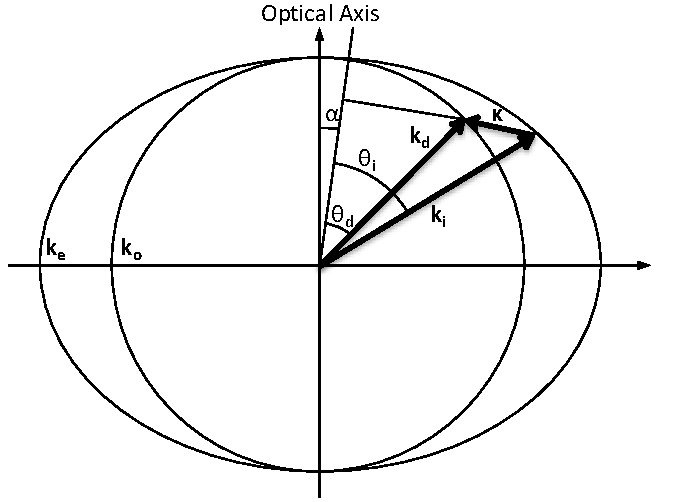
\includegraphics[width=0.7\textwidth]{./Images/3-1-AOTFWavevectorWithRefraction.pdf}
    \caption{The wave vectors generated by the AOTF experiment. From \autoref{eqn:3.1:phaseMatching}, the incident wave vector, diffracted wave vector, and acoustic wave vector are shown.}
    \label{fig:3.1:ATOFWavevectors}
    \end{center}
\end{figure}

\newpage

\begin{figure}
    \begin{subfigure}[t]{0\textwidth}
        \phantomcaption
        \label{fig:3.1:AOTFCharaterization:a}
    \end{subfigure}
    \begin{subfigure}[t]{0\textwidth}
         \phantomcaption
         \label{fig:3.1:AOTFCharaterization:b}
    \end{subfigure}
    \begin{subfigure}[t]{0\textwidth}
         \phantomcaption
         \label{fig:3.1:AOTFCharaterization:c}
    \end{subfigure}
    \begin{subfigure}[t]{0\textwidth}
         \phantomcaption
         \label{fig:3.1:AOTFCharaterization:d}
    \end{subfigure}
    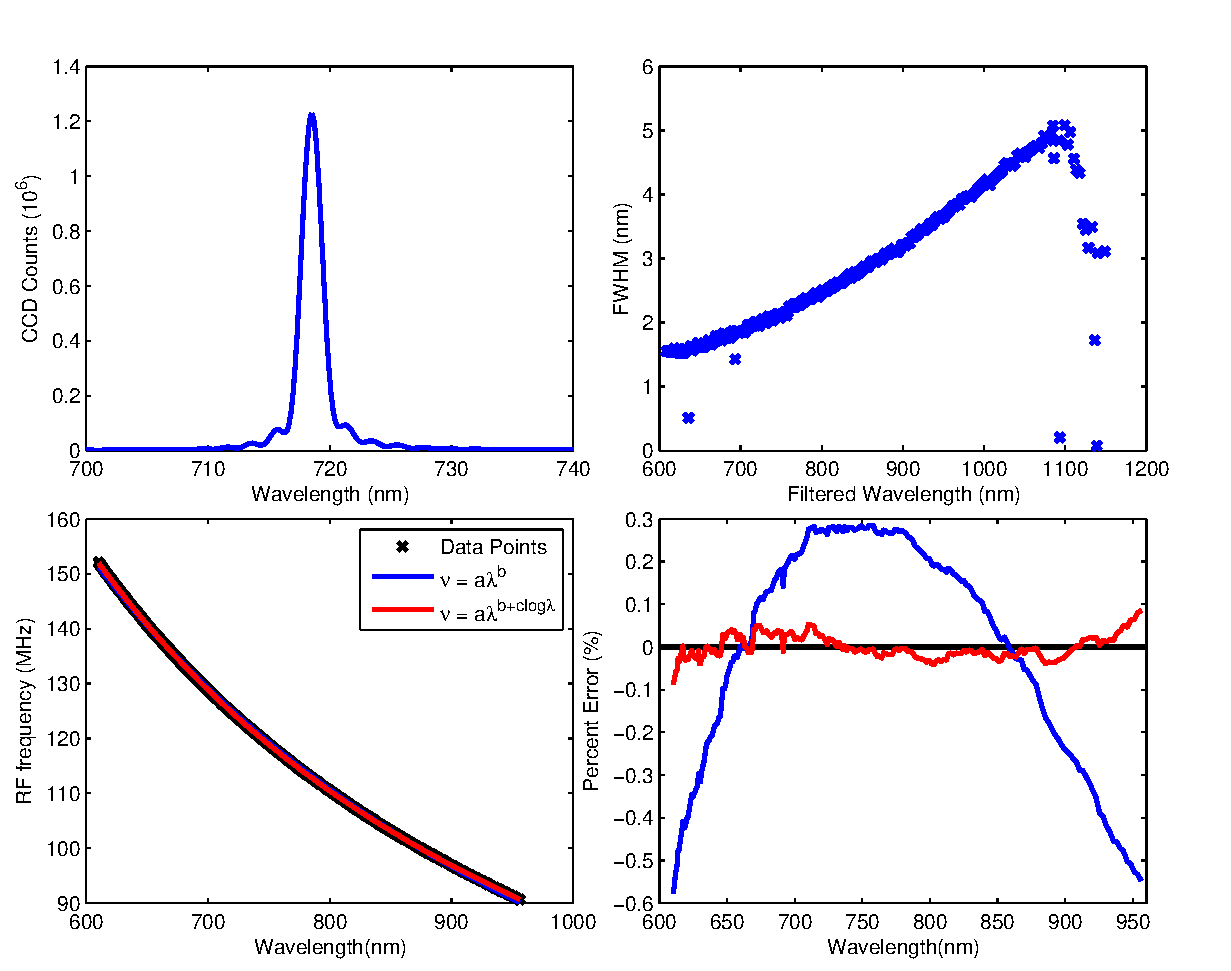
\includegraphics[width=1.0\textwidth]{./Images/3-1-AOTFCharaterization.pdf}
    \caption{(a) A standard image taken from the AOTF calibration experiment when the tuning frequency of the AOTF was at 124.96~MHz. (b) The FWHM for each of the determined wavelengths for the AOTF. The FWHM at 600~nm is 1.5~and as the wavelengths get longer the FWHM increases to 4.9 at 1080~nm. (c) The calibration curves for the AOTF RF versus the  diffracted wavelength which contains the data points recorded and two best fit curves. (d) The percent error with respect to the measured frequency for the two best fit curves in the previous panel.}
    \label{fig:3.1:AOTFCharaterization}
\end{figure}

\newpage

\begin{figure}
        \centering
        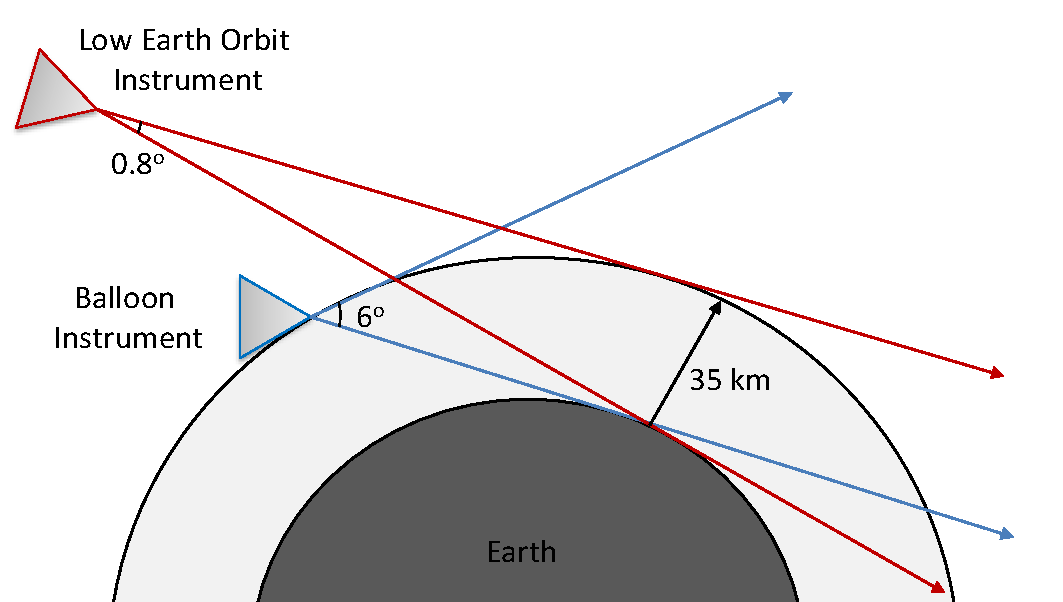
\includegraphics[width=0.75\textwidth]{./Images/5-4-BalloonGeometry.pdf}
        \caption{A comparison of ALI in a balloon and low earth orbit satellite geometries in blue and red respectively. In order to be able to gather the same vertical range of the limb a balloon geometry requires a 6\si{\degree} field of view at 35~km float altitude compared to a 0.8\si{\degree} field of view in a low earth orbit at 600~km.}
        \label{fig:5.4:balloonGeometry}
\end{figure}

\newpage

\begin{figure}
    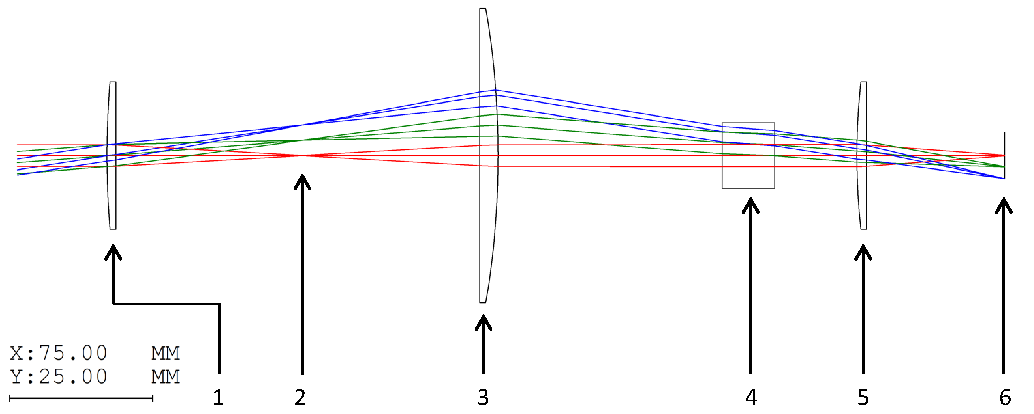
\includegraphics[width=1.0\textwidth]{./Images/3-2-TelescopicRayTracing.pdf}
    \caption{Ray Tracing diagram of the telescopic lens system for ALI simulated by Code V optical design software. The elements in the system are the following: (1) 150~mm focal length plano-convex lens. (2) Slit plate. (3) 100~mm focal length plano-convex lens. (4) Vertical linear polarizer. (5) Brimrose AOTF. (6) Horizontal linear polarizer. (7) 50.4~mm focal length plano-convex lens. (8) Imaging plane.}
    \label{fig:3.2:telescopicRayTracing}
\end{figure}

\newpage

\begin{figure}
        \centering
        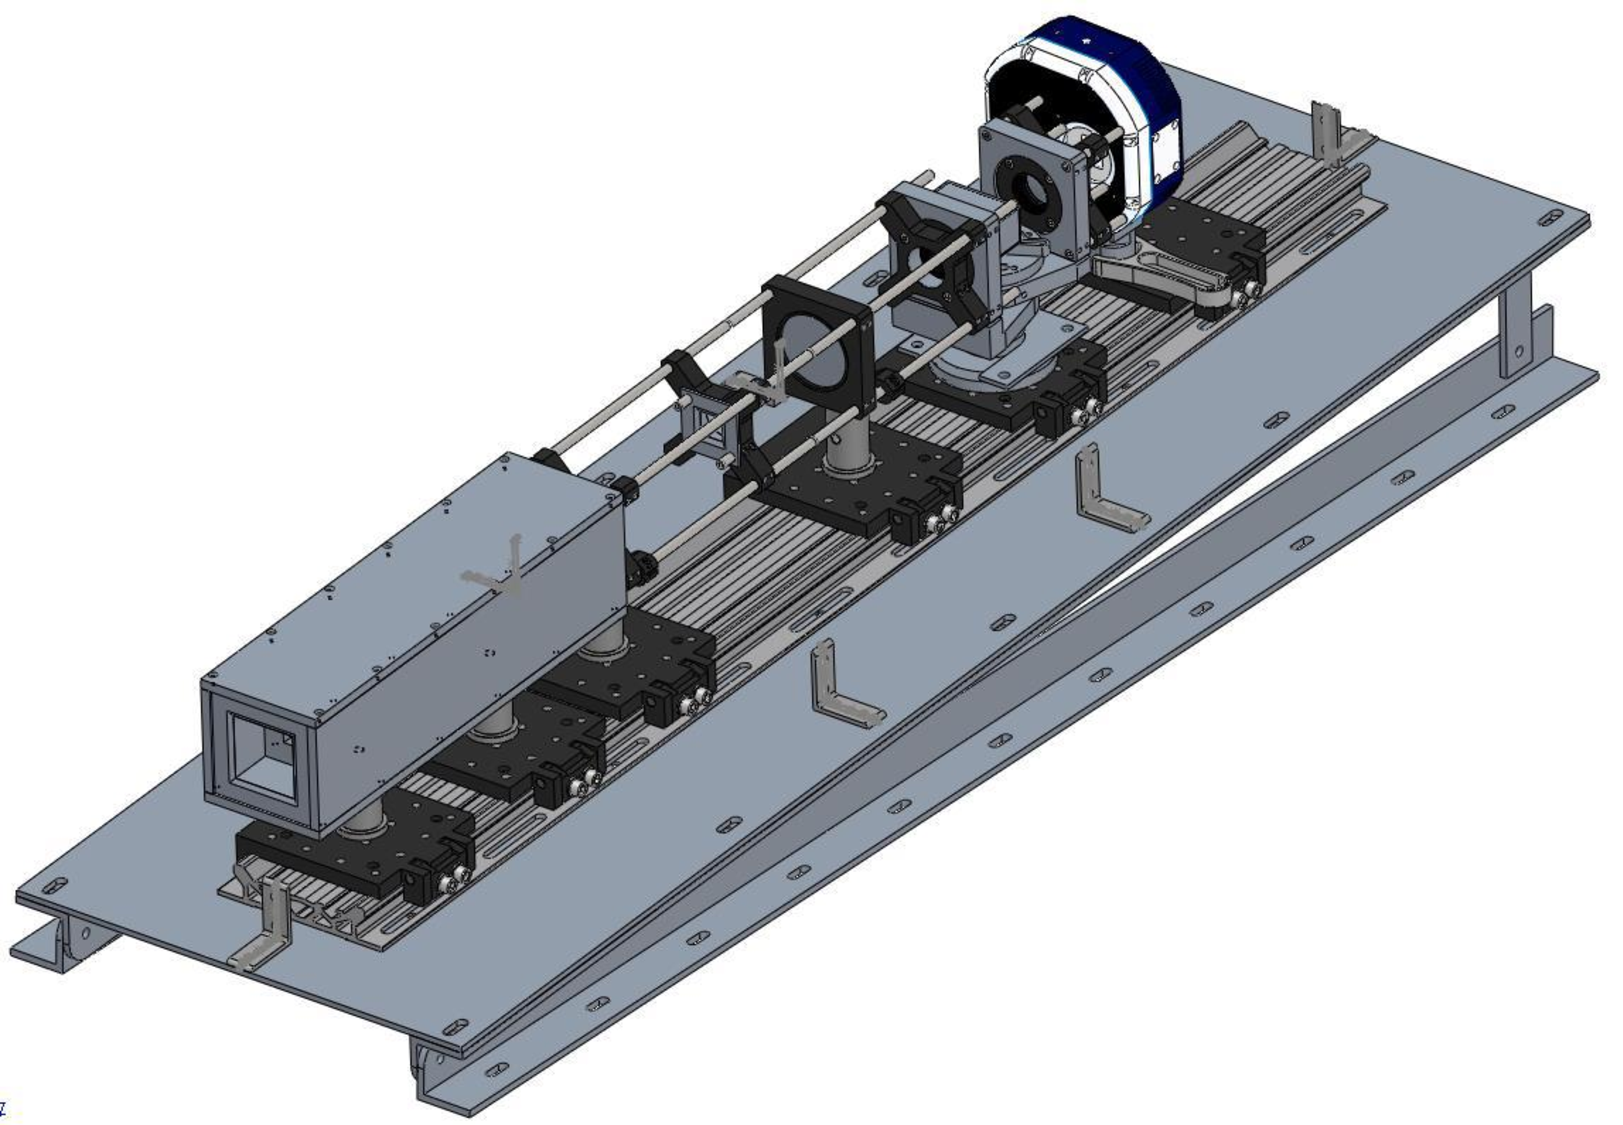
\includegraphics[width=1.0\textwidth]{./Images/3-3-AliCompleteDesign.pdf}
        \caption{An isometric view of the complete ALI system with the baffle and 3\si{\degree} slant required to correctly position the field of view. Light tight case absent from diagram.}
        \label{fig:3.3:aliSystemDiagram}
\end{figure}

\newpage

\begin{figure}
    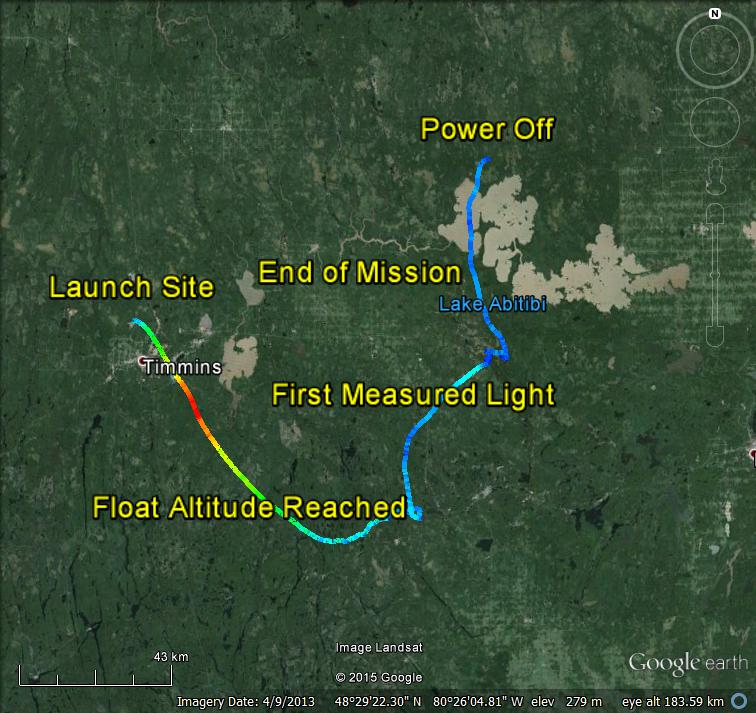
\includegraphics[width=0.42\textwidth]{./Images/5-1-AliGpsDataGoogleMaps.jpg}
    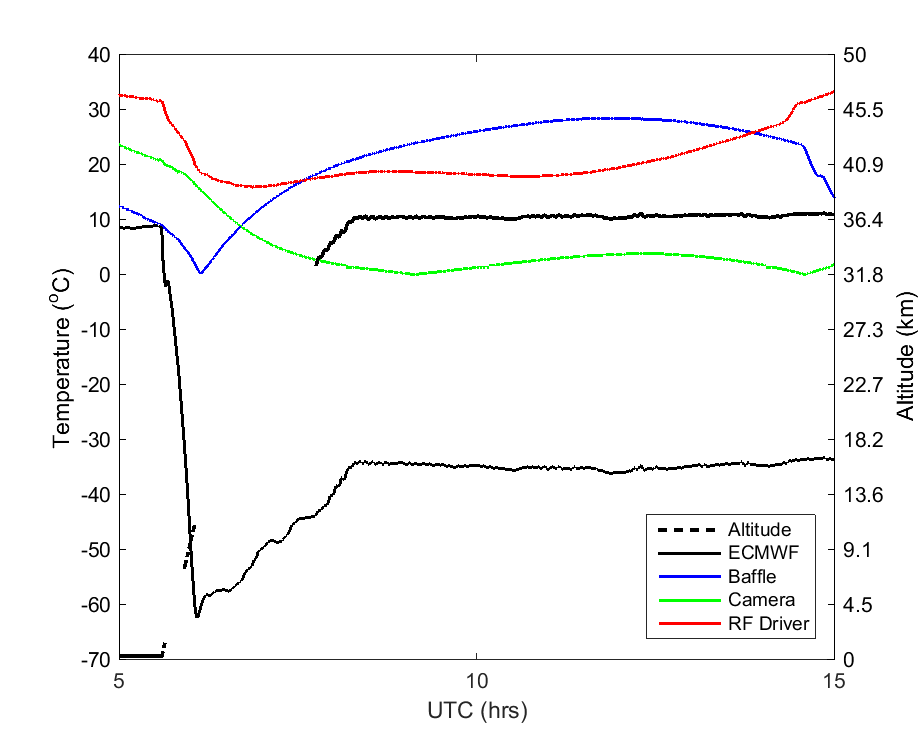
\includegraphics[width=0.52\textwidth]{./Images/5-1-FlightTemperatures.pdf}
    \caption{Left is the GPS data from ALI during the Nimbus 7 mission generated via Google Earth. The colour of the line represents the absolute speed of the gondola during the mission. Important landmarks are noted on the image. The end of mission represent the end of the aerosol mission. No GPS data was collected from ALI after power down. Right is the temperature and altitude profiles from the NIMBUS 7 flight.}
    \label{fig:5.1:nimbus7FlightPath}
\end{figure}

\newpage

\begin{figure}
    \begin{subfigure}[t]{0\textwidth}
        \phantomcaption
        \label{fig:AfterImagesHorizontalDependance:a}
    \end{subfigure}
    \begin{subfigure}[t]{0\textwidth}
         \phantomcaption
         \label{fig:AfterImagesHorizontalDependance:b}
    \end{subfigure}
    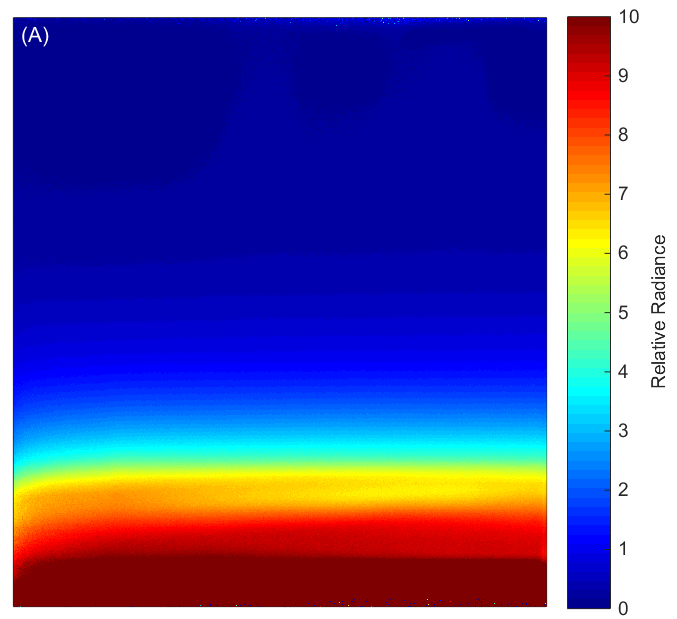
\includegraphics[width=0.52\textwidth]{./Images/5-2-AfterImage.pdf}
    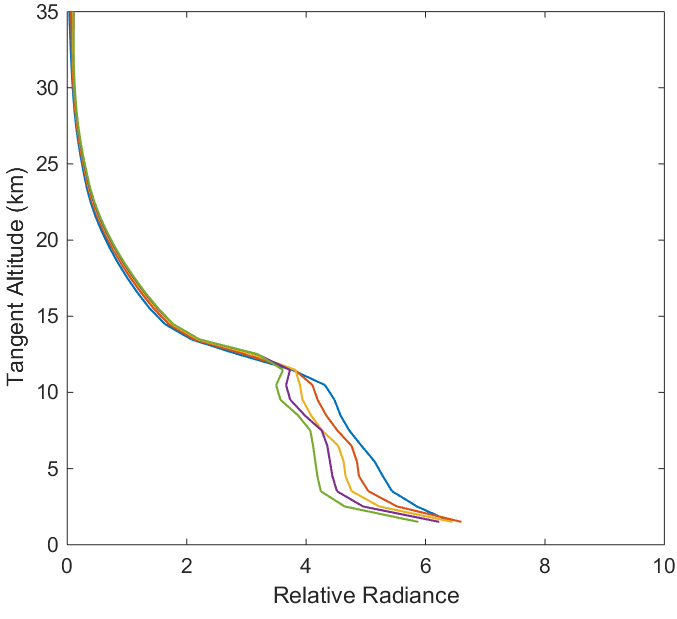
\includegraphics[width=0.45\textwidth]{./Images/5-2-AliRadiancesHorizontal.pdf}
    \caption{(A) Final calibrated 750~nm image, number 212. (B) The same 750~nm image as a with 5 horizontal line of sight shown to demonstrate horizontal dependance across the field of view.}
    \label{fig:AfterImagesHorizontalDependance}
\end{figure}

\newpage

\begin{figure}
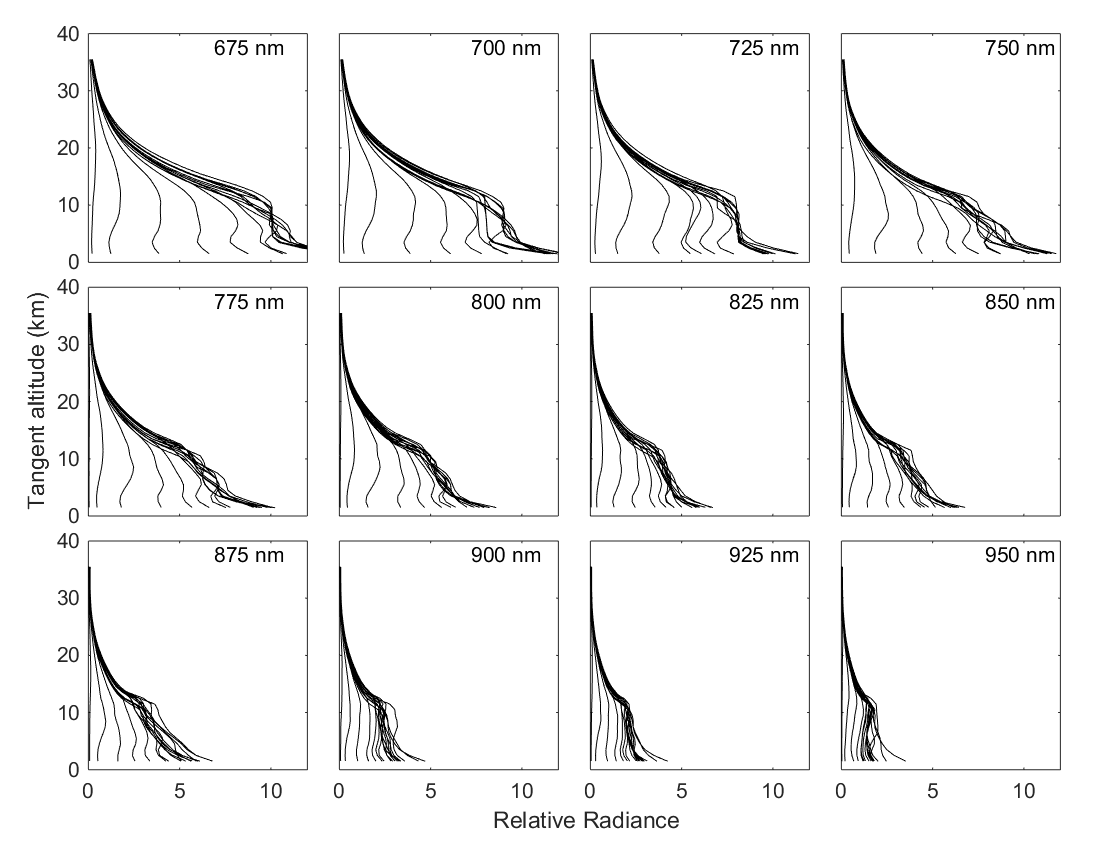
\includegraphics[width=1.0\textwidth]{./Images/5-2-AliRadianceVectors.pdf}
    \caption{All ALI relative radiance vectors from the NIMBUS-7 flight from the straight ahead line of sight, the average of the centre 25 columns of pixels, averaged to a 1~km resolution. Each panel presents the radiance vectors from a different wavelength measured which is denoted in the top right corner.}
    \label{fig:AliRadiancesVectors}
\end{figure}

\newpage

\begin{figure}
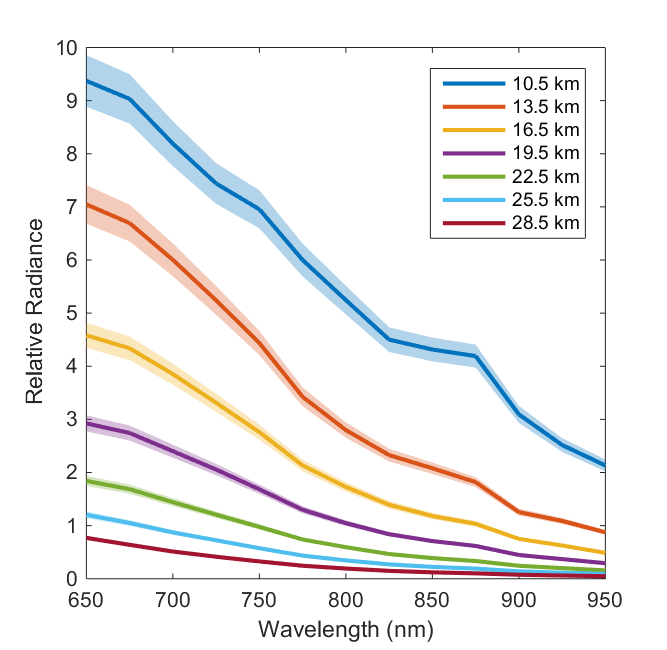
\includegraphics[width=1.0\textwidth]{./Images/5-2-AliSpectralRadiances.pdf}
    \caption{Level 1 relative radiances spectrally from 650~nm to 950~nm as measured from ALI at approximately 14:20 UTC consisting of images number 204 to 216 looking 90\si{\degree} from the sun facing southwards. These spectral profiles are presented at several tangent altitudes with a horizontal look direction of 0\si{\degree}. The shading represents the error on the radiances. }
    \label{fig:AliSpectralRadiances}
\end{figure}

\newpage

\begin{figure}
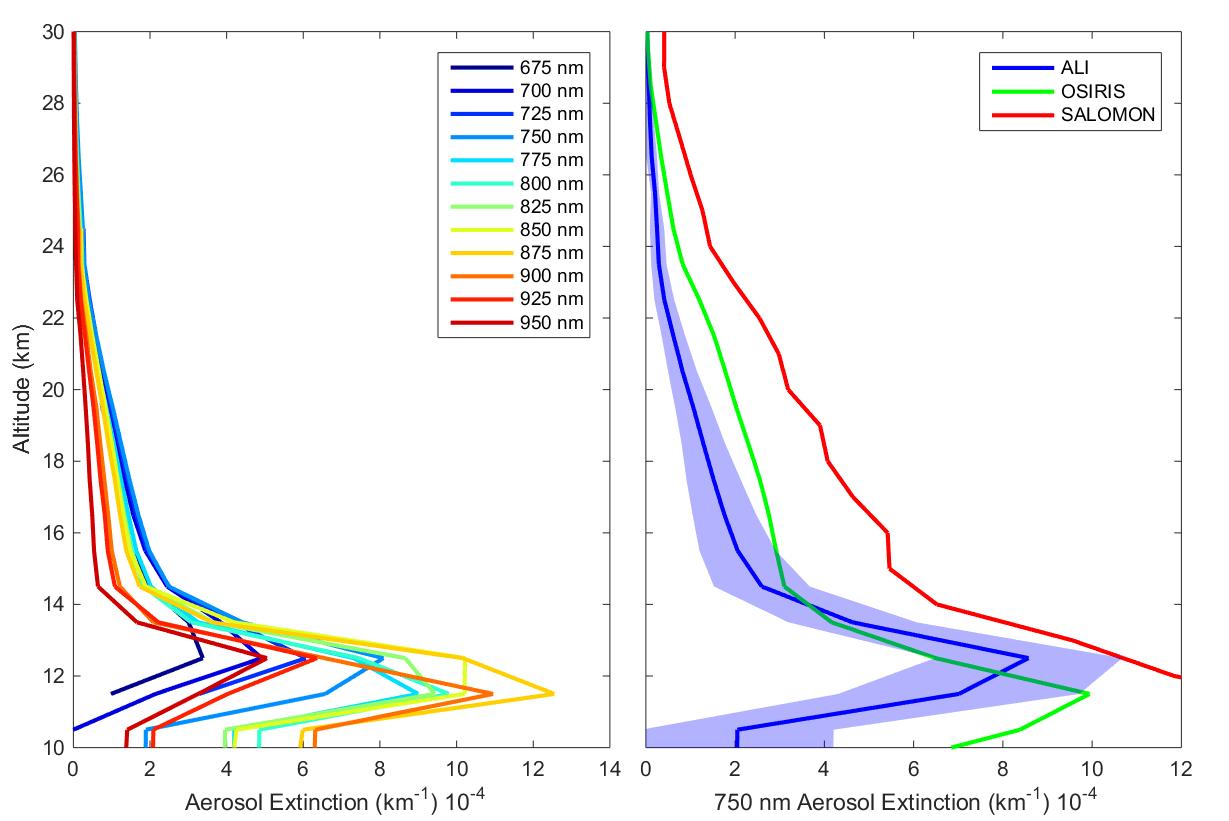
\includegraphics[width=1.0\textwidth]{./Images/5-3-FullAerosolCycleComparison.pdf}
    \caption{Left is the retrieved aerosol extinction profiles from the last complete imaging cycle consisting of images 205 to 216 from the 0.0\si{\degree} horizontal line of sight. Right is the 750~nm ALI aerosol extinction in blue with its error represented by the shading compared to the 750~nm extinction measured by OSIRIS and SALOMON in green and red respectively.}
    \label{fig:AliAerosolCycle}
\end{figure}

\newpage

\begin{figure}
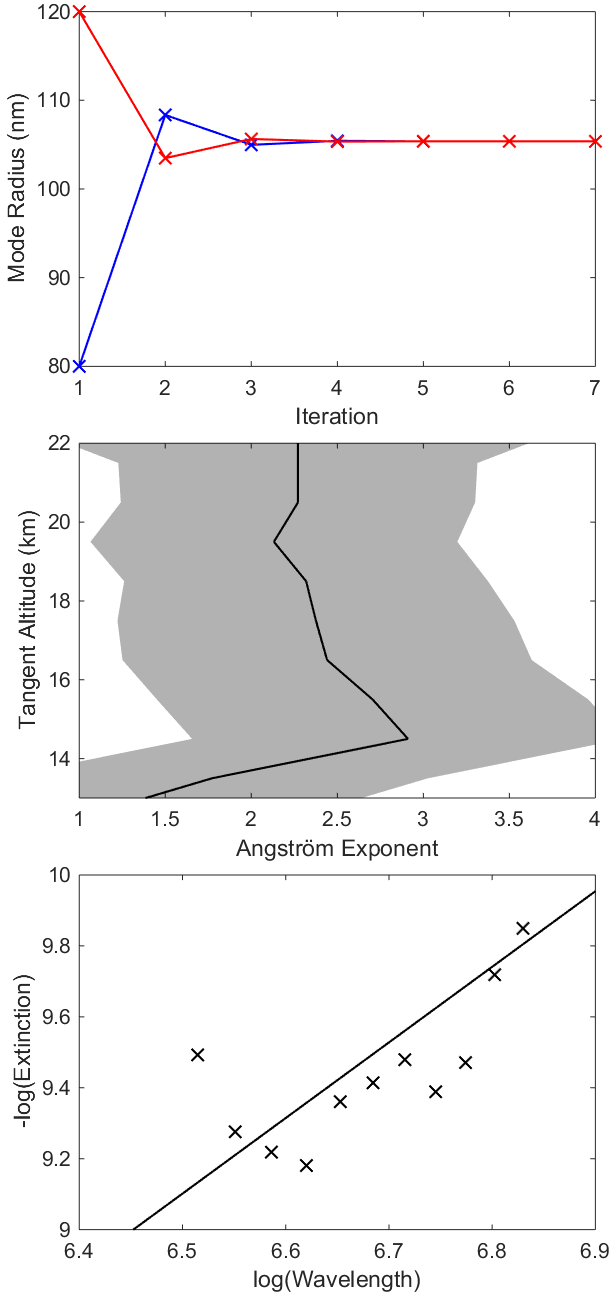
\includegraphics[width=0.5\textwidth]{./Images/5-4-ParticalSize.pdf}
    \caption{The top panel shows the convergence of two sample particle size retrievals over the iterations, blue and red represent a priori of 0.08 and 0.12~\si{\micro\metre} respectively. Both initial state converge to the same value over approximately 4 iteration in the particle size retrieval method. The second panel is the final Angstr\"{o}m exponents determined for images 204-217 during the Timmins 2014 campaign and are in black as the final profile was almost identical after each particle size retrieval, the shading represents the error associated with the least squares fit. The last panel demonstrate a least squares fit to determine the Angstr\"{o}m exponent at 20.5~km shell altitude.}
    \label{fig:ParticleSize}
\end{figure}

\end{document} 